\item \textbf{{[}NYJC/PRELIM/9569/2020/P1/Q1{]} }

\textbf{Figure 1} shows ten numbers stored in an array \texttt{L}.
\noindent \begin{center}
\begin{tabular}{|c|c|c|c|c|c|c|c|c|c|}
\multicolumn{10}{c}{\textbf{Figure 1}}\tabularnewline
\hline 
\multicolumn{10}{|c|}{\texttt{L}}\tabularnewline
\hline 
\texttt{{[}1{]}} & \texttt{{[}2{]}} & \texttt{{[}3{]}} & \texttt{{[}4{]}} & \texttt{{[}5{]}} & \texttt{{[}6{]}} & \texttt{{[}7{]}} & \texttt{{[}8{]}} & \texttt{{[}9{]}} & \texttt{{[}10{]}}\tabularnewline
\hline 
\texttt{34} & \texttt{8} & \texttt{6} & \texttt{35} & \texttt{27} & \texttt{35} & \texttt{63} & \texttt{56} & \texttt{16} & \texttt{24}\tabularnewline
\hline 
\end{tabular}
\par\end{center}

The numbers in \texttt{L} are to be sorted.

\textbf{Figure 2} shows an \textbf{incomplete} structure chart that
has been created while developing a solution to the problem of sorting
the numbers in \texttt{L}.

The constant \texttt{MAX} has been used to represent the size of the
array.
\noindent \begin{center}
\textbf{Figure 2} 
\par\end{center}

\begin{center}
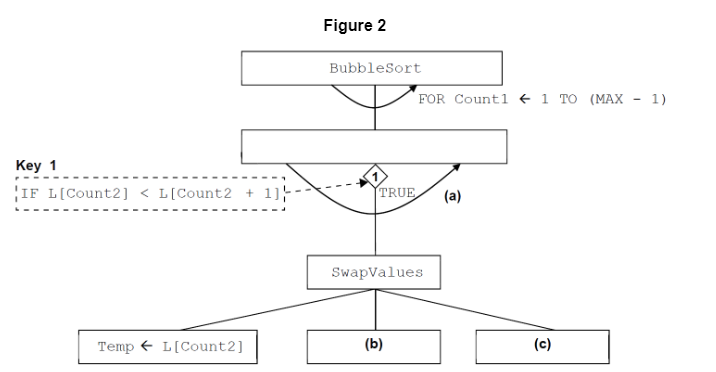
\includegraphics[width=0.5\paperwidth]{C:/Users/Admin/Desktop/Github/question_bank/LyX/static/img/9569-NYJC-2020-P1-Q1}
\par\end{center}
\begin{enumerate}
\item {}
\begin{enumerate}
\item Describe the goal of this problem. \hfill{}{[}1{]}
\item How should the curved arrow \textbf{(a)} in \textbf{Figure 2} be labelled?
\hfill{}{[}1{]}
\item What should be written in box \textbf{(b)} in \textbf{Figure 2}? \hfill{}{[}1{]}
\item What should be written in box\textbf{ (c)} in \textbf{Figure 2}? \hfill{}{[}1{]}
\end{enumerate}
\end{enumerate}
A new Bubble Sort routine is developed using the structure chart shown
in \textbf{Figure 2}.
\begin{enumerate}
\item[(b)] What value will be in \texttt{L{[}1{]} }when this Bubble Sort routine
has finished executing on the array \texttt{L} shown in \textbf{Figure
1}? \hfill{}{[}1{]}
\item[(c)]  A Bubble Sort routine, based on the structure chart in \textbf{Figure
2}, always completes \texttt{MAX - 1} passes through the array. Often,
this number of passes is not required, as the contents of the array
will be sorted after fewer passes have been made. If a pass is made
through the array during which no swaps need to be made, then the
array has been sorted.

Describe the changes that need to be made to the Bubble Sort routine
so that it will only complete the minimum number of passes through
the array that are needed to fully sort the contents of the array.
\hfill{} {[}3{]}
\item[(d)] The Bubble Sort routine can also be implemented using recursion. 
\begin{enumerate}
\item Define what is meant by a recursive function. \hfill{} {[}2{]}
\item Using pseudocode, write a recursive Bubble Sort routine.\hfill{}
{[}3{]}
\item Explain a disadvantage of a recursive Bubble Sort function over an
iterative one.\hfill{} {[}2{]}
\item Name and describe another recursive sort algorithm. \hfill{} {[}5{]}
\end{enumerate}
\end{enumerate}